\documentclass[english]{tktltiki}
\usepackage[pdftex]{graphicx}
\usepackage{subfigure}
\usepackage{url}
\usepackage{algpseudocode}
\usepackage{amssymb}
\usepackage{amsmath}
\usepackage{graphicx}
\usepackage{algorithmicx}
\usepackage[Algorithm,ruled]{algorithm}
\usepackage{float}


\DeclareMathOperator*{\argmax}{arg\,max}
\begin{document}
%\doublespacing
%\singlespacing
\onehalfspacing

\title{Big Data Influence Maximization blah balh}
\author{Behrouz Derakhshan}
\date{\today}

\maketitle

\numberofpagesinformation{\numberofpages\ pages + \numberofappendixpages\ appendices}
\classification{\protect{\ \\
A.1 [Introductory and Survey],\\
I.7.m [Document and text processing]}}

\keywords{layout, summary, list of references}

\begin{abstract}

Network influence maximization. Something about graphs, about network influcence, social network, other related areas, big data, hadoop and other technologies, graph processing

\end{abstract}

\mytableofcontents

\section{Introduction}
The term graph, first used by mathematician J. J. Sylvester, is a representation of set of objects, some of which are connected. Typically, in a graph the interconnected components are called \textbf{vertices}, and the links that are connecting them are called edges. Graph theory, is the field of mathematics that studies graphs and since its introduction, it has been used extensively, in many branches of science. In computer science, graphs can represents, networks of computers and the communication between them, it can represent websites and the links between them. In Chemistry and Physics, graphs are used to model the atoms and molecules and their interactions. In sociology, relation between actors, directors and movies can be depicted using a graph. And most notably is the its use case in social networks and modeling the relationship between people (friendship, acquaintance) . \\
Graphs components, can carry extra information, for example the edges can carry weight which can quantify or qualify the connection between two nodes. For example in a graph that represent geographical locations, where vertices (nodes) represent places, the edges represent the length between the locations. \\
With introduction of online social networks, an enormous amount of information is now available . One application that has been studied in social network or in graphs in general is the spread of information between nodes, based on the structure of the graph and the edge weights. In medicine and biology it has been used to find the spread of a disease either to find the initial person who contracted the disease or finding key vertices that could amplify the spread and by identifying those nodes further spread of the disease can be avoided. It has use cases in marketing as well, in which the aim is to find key people in a social network, that can spread the information among their friends and acquaintances, and for example by offering discount to a certain group of people they can rely on the work-of-mouth phenomena. \cite{kempe03} has defined models in which network propagation can be studied, and how to maximizes the the propagation in a network. \cite{domingo01} studied how to find the value of a customer in a network and how to use that to influence other customers. Influence maximization that is the topic of this thesis, has been studied for more than a decade now, but with the massive amount of available data, the scalability has become an issue. Some websites, such as Facebook, Twitter, Amazon, ... carry Terabytes and in some cases Petabytes of data related to their customers and their relationship. And the models developed for simulating the network propagation and finding the initial set that maximizes the influence, they will all suffer greatly when applied to graphs of this magnitude. \\
Over the past couple of years, many platforms for processing huge amount of data has been developed. This branch of computer science, named BigData, has gain a lot of attention lately. Some of the most notable frameworks are Hadoop and Spark. Hadoop is open source project that is based on Google's MapReduce framework. 
Using these and other similar frameworks, many graph processing tools and applications are built which utilizes the mechanism of these frameworks to process graphs of millions or billion of nodes and trillions of edges. \\
The most widely used frameworks for processing big graphs, are :
\begin{itemize}
\item 
Giraph which is open source project by on Google's Pregel framework. It is built on top of Hadoop
\item 
GraphX is open source project built on top of Spark
\item
Graphlab and open source project written in  and C++ . 
\end{itemize}

In this thesis, I will study the performance penalty of running state of the art algorithms for network propagation, more specifically the Independent Cascade method (which will be explained in the next section) . And propose and implement distributed methods for the algorithm written for GraphLab, GraphX and Giraph and comparison between each frameworks will be made. 
The rest of this document is organized as follow; in section 2, Big Data frameworks, graph frameworks, influence maximization methods are studies. In section 3, a distributed algorithm and implementation methods are presented. In section 4, comparison of the distributed and single node implementations as well as the difference between each graph framework are studied . In section 5 conclusion blah blah
In the next sections, different Big Data platforms are studied in details. Graph processing frameworks are explained extensively. And current and state of the art algorithms for network propagation and influence maximization are studied. 

\newpage

\section{Big Data}
Information and data has always been gathered for analysis and improvement or invention of new or existing technologies. It had helped governments to better govern countries, it had helped companies to better understand their costumers, and it had helped researchers and scientists to solve problems. With introduction of World Wide Web(http://webfoundation.org/about/vision/history-of-the-web/) exchange and collection of data has become a lot simpler. Big firms and companies started to collect user's information, browsing behavior and etc . Petabytes of data are being stored and exchanged everyday, and these data contain valuable information that is being used for solving a lot of problems using data mining and machine learning methods. 
Processing this amount of data, has never been an easy tasks and prior to introduction of new BigData technologies, this processing and analyzing has been always done using expensive Server systems that are able to process millions to billions of bytes of data in a second. 
Google Inc. revolutionary papers has drastically changed field. \cite{ghemawat03} introduced \textbf{The Google's Distributed System}; a file system built for storing terabytes of data. It is scalable, meaning more storage can be easily added, and it is being deployed on commodity hardware, meaning it does not require any sophisticated and expensive piece of hardware to use. Dean et. al \cite{dean04} introduced \textbf{MapReduce} a framework for processing large amount of data, again it is scalable and it can be deployed on commodity hardware. 
Although the source code either of these two technologies were never released by Google, but based the publications \textbf{Doug Cutting} created the open source project \textit{Hadoop} which implements both MapReduce (Hadoop's MapReduce) and Google File System (Hadoop Distributed File System or HDFS for short). Since then, Hadoop has become BigData standard, several new technologies and project have been added to it.

\subsection{Hadoop}
Hadoop is consists of two major parts. 
\textbf{MapReduce} which is a parallel programming paradigm. It is designed to run on distributed systems with many commodity computers. It involves three main steps, namely \textit{Map}, \textit{Reduce} and \textit{Shuffle}. The first two are defined by the user. Map operations are run in parallel and they process the data individually, data is divided into different portions and each one is processed by a mapper. The result of the mappers are send to a Reduce task(or several) where the results are combined. A shuffle operation is usually performed on the result of the Map tasks so that similar data are all send to the same nodes. Below is a simple algorithm for counting words in a series of documents. 

\begin{algorithm}
\begin{algorithmic}
\Function{map}{String name, String document}
\State {//name: document name}
\State{//document: document contents}
   \For {each word w in document}
      		\State emit (w, 1)
   \EndFor
\EndFunction
\State 
\Function {reduce}{String word, Iterator partialCounts}
\State{//word: a word}
\State{//partialCounts: a list of aggregated partial counts}
  \State sum = 0
  \For{ each pc in partialCounts}
    \State sum += ParseInt(pc)
    \State emit (word, sum)
\EndFor
\EndFunction
\end{algorithmic}
\end{algorithm}

\begin{figure}[ht!]
\centering
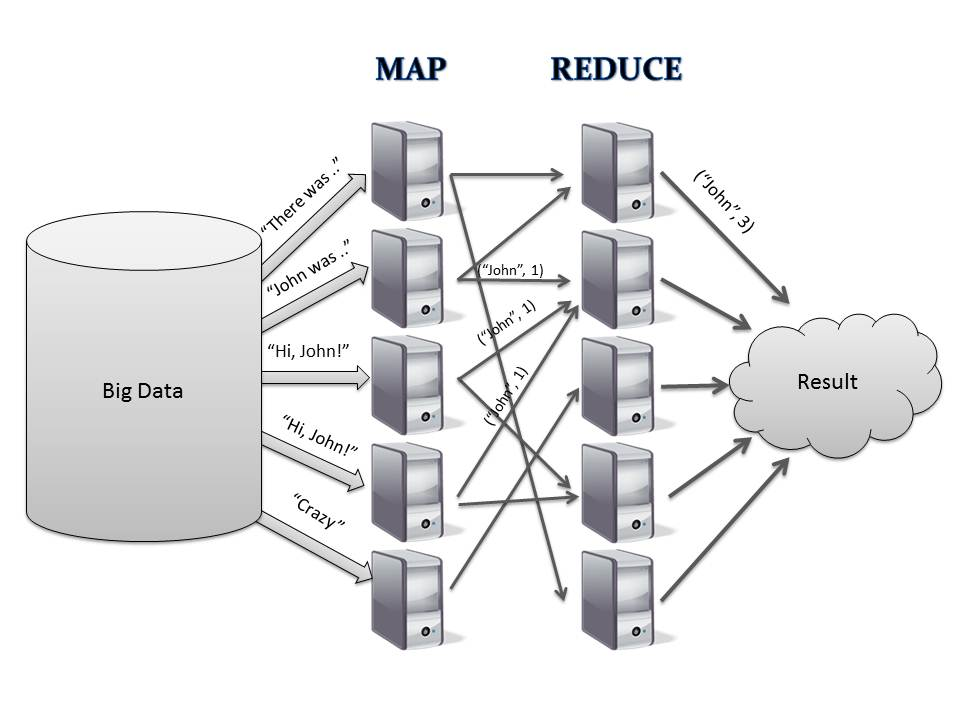
\includegraphics[width=130mm]{figures/mapreduce.jpg}
\caption{MapReduce paradigm}
\end{figure}

The popularity of Hadoop's MapReduce framework rises from the fact that many complexities of the system is being handled automatically by the framework. In most typical use cases, the user only needs to provide the method for Mappers and Reducers. Framework will take care of compiling and distributing the code to all the nodes, and running them in parallel. As previously mentioned it is fault tolerant, it means if during the processing a task fails, it will restart the task again, if a node encounters a problem the framework will move the computation to another node. It is scalable, which means the program does not need to know how many nodes are involved in the system. The program will scale to many nodes depending on the size of the input data and amount of available resources. There are however many advanced options that users can do to further optimize the program, but they are generally not required for simple tasks. The other feature of MapReduce and Hadoop in general is that it is available in many different languages. Java, Python, C++, Scala and many more. 

Newer versions of Hadoop and MapReduce employs more sophistcated Resource manager and Scheduler called YARN(TODO REFERENCE) . YARN essentially, provides container for running different applications and it is not limited to MapReduce. Spark, Storm and and even simple Java programs can be run on YARN. YARN is more or a less cluster manager program and overviews the resource and allocates resources to different jobs being submitted to it. It has become available as part of Hadoop 2.0 technology Stack .

\textbf{Hadoop Distributed File System (HDFS)}
HDFS is a distributed file system, designed to run on commodity hardware. It provides high throughput access to application data and it fault tolerant. Though initially designed for Hadoop's MapReduce framework, it has been used in many different application.
\begin{figure}[ht!]
\centering
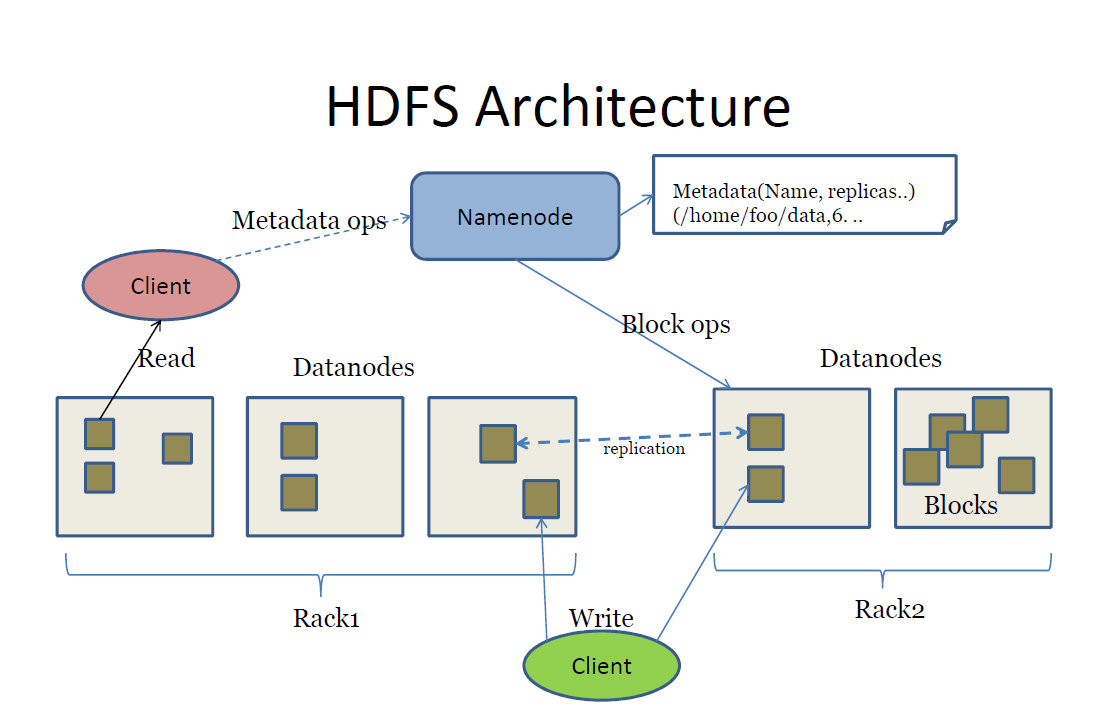
\includegraphics[width=130mm]{figures/hdfsarchitecture.png}
\caption{HDFS Architecture}
\end{figure}

It is fault tolerant, meaning if a node in a cluster fails, the data is not gone. HDFS employs a feature called \textit{Data Replication}, which indicates the number of type each object is being replicated. NameNode keeps track of where are all the same instances of the data is stored and in case a node fails it knows where to look for it. HDFS emphasizes on moving computation is much cheaper than moving data, it is true since HDFS is designed to store BigData sets, Tera or even PetaBytes of data, hence in conjunction with MapReduce, instead of moving the data around, the computation is done on the node containing the data. It is design for high throughput  rather than low latency so it is not ideal for streaming application, although several improvements are being made to further decrease the latency and making it suitable for real time streaming application. Similar to MapReduce it is design to work across heterogeneous hardware and software platforms. Meaning the nodes in the cluster do not have to be identical and even running the same operating system. Hadoop runs on JVM hence it is OS agnostic. 


\subsection{Spark}
Apache Spark \cite{zaharia10} was originally developed in AMPLab at UC Berkeley. The main idea was to solve MapReduce's problems. In contrast to MapReduce's 2 stage program (Map and Reduce), Spark employs an iterative paradigm. It allows users to load data into memory and perform many operations on the data, this is ideal for a lot of Machine learning problems. The underlying frameworks work on entities called Resilient Distributed Datasets (RDDs) \cite{zaharia12}. RDD  is a read only and partitioned collection of data. It can be created from storage or other RDDs. There two types operation on RDDs, transformations and actions. Transformations are operations that will create a new RDD from the existing one, for example \textit{filter}is a transformation operation. The power of RDDs lie in their internal structure, they do not need to be materialized all the time. If a RDD is created using a transformation, it will hold information about how the transformation was made and only apply them to the data once the user requests that through an action or caching the data set. Actions are operations that will materialize the dataset. Users can also ask the RDD to be stored in memory if they know they are going to use its value many times. These characteristics of RDD makes the perfect tool for performing iterative applications. Many machine learning algorithms require iterative calls to the same dataset. This is one of MapReduce's deficiency since every algorithm and job has to be written in terms of Map and Reduces. Spark with the help of RDDs allow many of the well known machine learning algorithms to be applied to without much change to actual algorithm. With success of Spark, it had become part of the Hadoop framework. Recent versions can now on top of Yarn and they have integration with HDFS and other Hadoop components. 
A typical Spark program is consists of a driver program that launches multiple workers. Worker programs are run on data nodes. upon execution of a program, Spark will try to send the computation to where the data is, hence minimizing the network traffic. Spark tracks where the RDDs and their partitions are.
\begin{figure}[ht!]
\centering
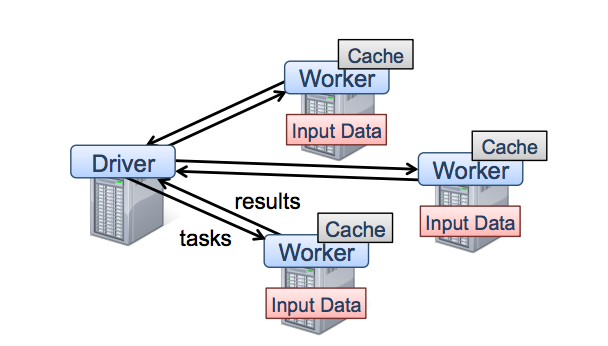
\includegraphics[width=130mm]{figures/sparkprogram.png}
\caption{Spark Program}
\end{figure}

 User's can control RDDs behavior by persisting it, or caching it. Tests performed on Spark showed that it is 100x times faster than MapReduce and it is able to run application that are not even possible to run using MapReduce. Spark is fault tolerant by means of RDDs. Since RDDs track the changes made to them, they can be recreated. So if a node containing some partitions of RDDs are lost they can be recreated using the these information. 
 
\begin{figure}[ht!]
\centering
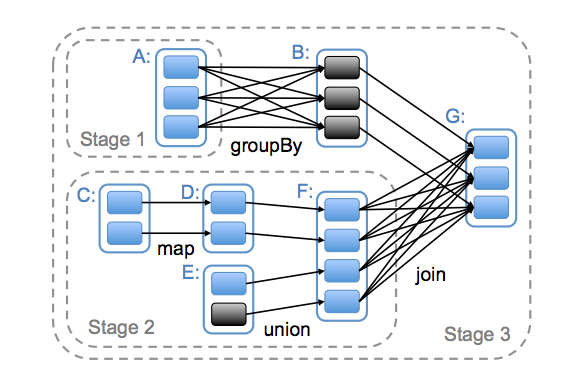
\includegraphics[width=130mm]{figures/rdd.png}
\caption{Spark stages and RDDs}
\end{figure}
Figure above shows how Spark computes job stages. Boxes with solid outlines are RDDs. Partitions are shaded rectangles, in black if they are cached. To run an action on RDD G, the scheduler builds stages at wide dependencies and pipelines narrow transformations inside each stage. In this case, stage 1 does not need to run since B is cached, so we run 2 and then 3. If any of the stages fail, the computation will restart from the last healthy RDD. Also if a node containing some specific partitions of an RDD fails, the RDD will be transferred to another node and the computation will be restarted. 

Spark contains a Machine learning framework named MLib and graph processing framework named GraphX . 
Spark works very well with iterative algorithms, it doesn't have MapReduce limitation which is the result of each job has to be written to disk. Spark has in memory computation which will speed up the process. 
% Spark Word Count Problem in Java and Scala

\section{Big Graph}
What is it, where does it come from, why is it important to have frameworks capable of processing massive graphs

\subsection{Giraph}
Apache Giraph is an iterative graph processing framework, built on top of Apache Hadoop. It is the open source version of Pregel by Google \cite{malewicz10} . Its input is a graph consists of vertices and edges. Each vertex and edge contains value as well, hence the input to a \textbf{Giraph} program besides from the structure of the vertices and edges includes their initial values. The project is now being actively developed by several companies. It is being used in many real case scenarios. For example, Facebook is using it to analyze the graphs formed by users and their connection with their friends. Similar to Pregel, the computation model of Giraph is Bulk Synchronous Parallel \cite{valiant90}. A BSP computation model consists of three physical components : 
\begin{itemize}
\item
A component capable of local processing
\item
A network for transferring messages
\item
A hardware which synchronizes the components
\end{itemize}
BSP programs are run in parallel on each processing components and then the messages are transferred between these nodes. All of the computations are done in steps and after each step is done all the components should wait until every other component have finished its processing and sends messages to other components. \\
The architecture fits very well with BigGraph computations in a way that vertices will process data individually and send messages along the edges (or directly) to other vertices in each step. The process can be parallelized then so that all or as many vertices as possible will perform computation at the same time and send messages and at the end of each step (which is called a super step in BSP) they will wait to synchronize with other vertices. 
The computation will continue until all vertices are inactive or no more messages were sent during a step. This figure shows the general process in BSP models : 
\begin{figure}[ht!]
\centering
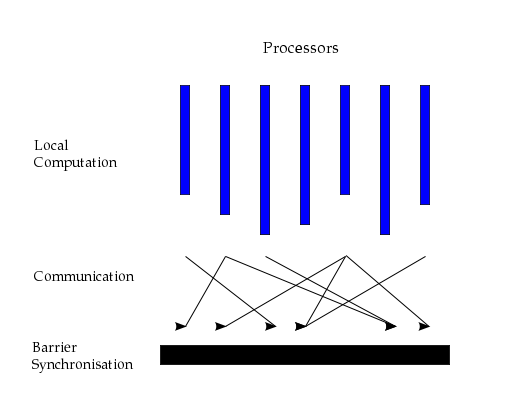
\includegraphics[width=130mm]{figures/bsp.png}
\caption{Bulk Synchronous Parallel}
\end{figure}

Based on BSP, Giraph first distribute all the vertices to different nodes, users can define the partitioning behavior so it would suite the specific kind of algorithm they are going to run. Generally the idea is to have vertices that are connected on the same node, since most of the communications are done through edges and hence this would minimize the network traffic across the cluster. Computation then begins in a series of super steps, in each one messages from the previous super step are gathered by each vertex, the vertex will do its computation and send new messages to other vertices, at the end of the each superstep, all the vertices are synchronized, counters that keep track of the status of the cluster are updated, users can also define counters and aggregators. For example, finding the vertex with the maximum value in each iteration or etc. Giraph has a series of built in aggregators and users can define their own. At the end of the computation vertices can send a command to master node telling it that they'd like to halt and done computing, their state is changed to in active and it will stay like that unless new messages are sent to those vertices. When all the vertices are in active the computation will halt and the result will be reported.
Figure below shows how computation is done in Giraph . (TODO, source or create your own graph)
\begin{figure}[ht!]
\centering
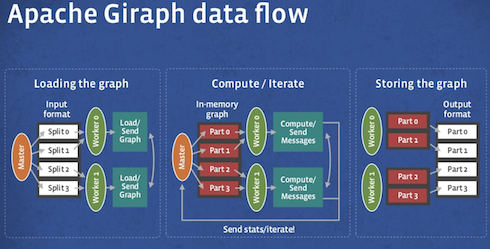
\includegraphics[width=130mm]{figures/giraphdataflow.png}
\caption{Giraph Work Flow}
\end{figure}
A typical Giraph program is carried out in several steps, each one called a \textit{superstep} . Initially all vertices are in an \textit{active} state, and each iteration an active vertex will call its compute method which is defined by the user and generally carries out the Giraph algorithm. A typical Compute method:
\begin{itemize}
\item
receives messages sent to the vertex in the previous superstep
\item
computes using the messages, and the vertex and outgoing edge values, which may result in modifications to the values, and
\item
may send messages to other vertices.
\end{itemize}

The figure below shows supersteps involved with computing the single source shortest path for a simple graph.(TODO, make your own proper reference)
\begin{figure}[ht!]
\centering
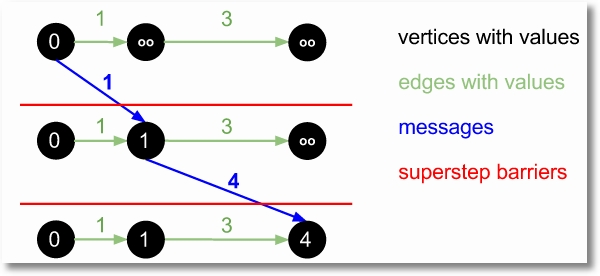
\includegraphics[width=130mm]{figures/giraphsuperstep.jpg}
\caption{Single Source Shortest Path}
\end{figure}

The input is a chain graph with three vertices (black) and two edges (green). The values of edges are 1 and 3 respectively. The algorithm computes distances from the leftmost vertex. The initial values of vertices are 0, $\infty$ and $\infty$ (top row). Distance upper bounds are sent as messages (blue), resulting in updates to vertex values (successive rows going down). The execution lasts three supersteps (separated by red lines).

On a cluster level, a graph is distributed into several connected components and each one is stored in one of the computation nodes. Each cluster, has a master node that coordinates the other nodes. It will decide on which components should be stored on each device and it stored reference and tables of information about the vertices and edges and where they resides. It will ensure the supersteps are synchronized, i.e. it makes sure all vertices have finished their computation in the current superstep before starting the next superstep. It will monitor the status of the components and decide when to end the program by checking if there are any active vertices or not. 
Although it has many advantages over MapReduce, it is still has many limitations, in one Giraph job many iterations can be done, but if graphs should go through several transformation that would require multiple Giraph jobs, which means that the data has be written to HDFS after each job which adds overhead. A lot of the Machine learning and graph algorithms and problems are iterative in nature, which will cause Giraph to have severe performance issues in some of these cases. 
% Sample code 
\subsection{GraphX}
% Where did it come from
% Advantages over Giraph and traditional MapReduce and Spark
% Limitations 

\newpage

\section{Influence Maximization}
Effective marketing and advertisement methods has been a major application of Knowledge Discovery and Data mining. Prior to \cite{domingo01} the focus has always been on direct marketing. Contrary to traditional mass marketing, where a product was marketed to all the customer, in direct marketing the goal is find the most potential and profitable costumers.  One example is \textbf{Recommendation Systems} which based on users previous purchasing habits will recommend new items. While direct marketing is a great tool for increasing the profit, it only targets individuals and disregards the relationship between users. People's decision in purchasing an item is not only influenced by the product itself, but also by friends, colleagues and acquaintances. With introduction of Internet and Social networks, gathering information about users became easier and more feasible. Social networks nowadays contains information about millions of people, they also contain information related to people's relationship with each other. Utilizing these information, can make marketing more profitable, by targeting people that are more likely to promote the product to their acquaintances. 
\cite{domingo01} discussed the use case of influence maximization in marketing, calling it \textbf{Viral Marketing}. By modeling a market as a social network consisting of users and products. In such a network, probability of users buying products only depends on the product itself, the neighbors of the user and the set of marketing actions being applied to the network. Hence the market can be formulated as join probability distribution. 
Through these a function was devised that calculates the global lift in profit given a marketing action was applied to some users. Starting from an initial configuration, using different optimization algorithms a local maxima for the function can be reached. Hence the problem of influence maximization can be formulated as follows. \\ \\
\textit{Given a size $k$ for the initial seeds, find the set of nodes $A$ that maximizes the function $f$ which is the size of spread through out the network . }\\ \\
They experimented on a collaborative filtering data set (MovieLenz) in which users have rated a list of movies. They have first constructed the network with the user ratings, by choosing similar users(calculating the Pearson correlation coefficient of users) as neighbors . They have performed experiments on the data set and compared their method with mass marketing and direct marketing. Their method has increased the profit the most. Due to non-linearly of the model, it did not scale well for bigger size networks, hence they have proposed a new linear model \cite{domingo02}. Not only the new model decreased the computation time, they simplified equation for calculating the network value of customers, made it easier to incorporate more complex marketing action. They have experimented with Epinions \footnote{http://www.epinions.com/}data set. Which is a website where users can rate items. It also has a feature called trusted users, where each user can select many other users as trusted sources of reviews. Domingo et .al, hence, applied their model to the dataset, by considering trusted users of a user his neighbors. Their experiments showed that a continuous marketing action (a marketing action that can have unlimited values, such as a discount) performs much better than boolean marketing actions (one that can either be true or false, such whether or not a discount should be given to a user with no regards for the amount of the discount).  
\subsection{Information Diffusion Models}
With introduction of Social Networks, the topic of information diffusion has gain interest in research community. Information diffusion models describe how information and data are being propagated and transferred in social networks. Information diffusion is not only limited to social networks, for many years the topic has been studied to better understand for example how a disease is being spread among people or how contaminated water would affect a water pipe network. In influence maximization Kempe et .al \cite{kempe03}  studied two important information diffusion models.
\begin{itemize}

\item Linear Threshold Model :\\
Consider a directed graph G representing a social network, and individual nodes being either active or non-active. Inactive nodes may become active as more of their neighbors become active but the reverse is not possible. In \textit{Linear Threshold Model} each node $v$ is influenced by each of their neighbors $w$ according to a weight $b_{v,w}$ such that $\sum \nolimits_{w \, neighbor \, of \, v} b_{v,w} < 1$ . The diffusion process hence is as follows; each node $v$ will randomly chose a weight threshold $0 < \theta_v<1 $, this value determines tendency of node $v$ to become active. Starting from the initial seed set, in each iteration for each node if the sum of the weights of its active neighbors is greater than the threshold then the node will become active, i.e. $\sum \nolimits_{w \, active neighbor \, of \, v} b_{v,w}  \geq \theta_v $. The process is deterministic however since $\theta_v$ is chosen at random, it shows our lack of knowledge of their values. This process continues until no new nodes become active.

\item Independent Cascade Model :\\ 
 \textit{Independent Cascade Models} is a stochastic undeterministic process. Same as \textit{Linear Threshold Model}, it starts with an initial set of seeds, and in each time step $t$ every active node will try only once to activate all of its neighbors, the probability of a node $v$ activating one of its neighbors $w$ is define by a system property $p_{v,w}$. The process continues until no more new node can become active. Every node will try to activate its neighbors independently of other nodes, and if during one time step, a node $v$ first becomes active by node $u$ the rest of $v$'s neighbors can skip the activation process. In that sense the ordering of which nodes should to activate their neighbors first does not matter and it will not affect the final result.
\end{itemize}
Based on \textit{IC} different models have been also discussed, such as \textit{Weighted Cascade} which is similar to \textit{IC} with the exception of the activation probability. Where in \textit{IC} it is defined as a global property, in \textit{Weighted Cascade} each edge from $u$ to $v$ is assigned the probability $1/d_v$, where $d_v$ is the degree of vertex $v$. The probability for edges in weighted methods can be calculated in different ways, in fact finding the influence of nodes on each other is another research area in influence maximization and it is briefly explained in \ref{subsec:learninginfprob} .

\subsection{Influence Maximization Problem}
Kempe et .al \cite{kempe03} were the first to formulate Influence maximization as an optimization problem and prove that the problem is NP-complete. By studying how influence propagates through networks, they discussed two diffusion models \textit{Linear Threshold Model} and \textit{Independent Cascade Model}. They have formally expressed Domingos and Richardson's \cite{domingo01} optimization problem in the context of the above models. Both models involve an initial set of nodes $A$, the influence of a set $\sigma (A)$ is then defined as the number of nodes at the end of the process. Finding the optimal set is NP-hard but they proposed an approximation algorithm for the problem which guarantees the solution to be a factor of $(1 - 1/ \mathrm{e} - \varepsilon)$ of the optimal solution (slightly better that 63\%). 
Approximate solution for these models is developed based on \textit{submodular functions} \cite{nemhauser78}.
A function $f$ is \textit{submodular} if it satisfies a natural ''diminishing returns'' property. It means the marginal gain of adding a node $v$ to a set $A$ is always greater than or equal than adding $v$ to a super set of $A$ . 
\begin{center}
$f(A \cup \{v\}) - f(A) \geq f(S \cup \{v\}) - f(S)$, where $A \subseteq S$
\end{center}
The greedy algorithm proposed by Kempe i \cite{kempe03} is as follows 
\begin{algorithm}[ht!]
\floatname{algorithm}{Influence Maximization}
\caption{Greedy Algorithm}
\label{alg:KempeInfMax1}
\begin{algorithmic}
\Require k,G(V,E)
\State A = $\emptyset$
\For {i = 1 to k}
	\For {every $v \in V$ and $v \notin A$}
		\State $\delta_v = \sigma(v)$
	\EndFor
	\State $v^* = \argmax_v \{\delta_v\}$
	\State $A = A \cup v^*$
\EndFor
\end{algorithmic}
\end{algorithm}
They have run experiments on co-authorship in physics theory section of arXiv \footnote{www.arxiv.org}. The results show that their greedy algorithm performs better that other methods such as random selection, high-degree or central nodes .
Both in estimating the spread and also in the greedy method, $\sigma (A)$ has to be calculated, but both of the propagation models are non-deterministic. To overcome this, the model is run many times (10000 times) and the spread is the average of all the runs. The nature of the spread function makes the algorithm highly non scalable. Even on medium sized graphs running the simulation thousands of time will take a lot of time, but on the other hand a good solution is only guaranteed if the simulation is run many times. From Algorithm \ref{alg:KempeInfMax1} it can be observed that $\sigma(v)$ is run for every node in every iteration, this will greatly affect the performance of the greedy method.
Leskovec et .al \cite{leskovec07}  in their Cost effective outbreak detection in networks, took upon the task of optimizing the greedy method used in propagation in graph networks. Although they did not work on solving the problem of maximizing influence they have proven their method can be adapted to the problem of maximizing the influence using the greedy algorithm. They studied two problems from different domains which share similarities. The first problem is find the best placement of sensors in a water network, so that contaminated water can be detected as quickly as possible. The other problem is blog network, which is to find blogs that contains the maximum amount of news that cascades from different sources in shortest possible time. Their advanced greedy method, called CELF, utilizes the submodularity of the objective function, which reduces the amount of computation needed to be made in each iteration. Their method is 700 times faster than a simple greedy function. 
Their observation is that, if A is subset of B, the marginal gain of adding a node to B is always less than or equal to the marginal gain of the adding the same node to A. Hence instead of recomputing the gain for all the node in each iteration, we can go through the nodes in decreasing order of their spread and recompute their values, the change is usually very small and most of the time the value on top of the list stays on top. 
\cite{chen09}proposed several different methods for solving the problem of Influence Maximization. The first group of algorithms, were improvement upon Kempe \cite{kempe03} and Leskovec \cite{leskovec07} greedy method. In their greedy method, they have modified the simulation process. Instead of trying to activate nodes based on the edge probability one by one, they have first created a new Graph $G'$ which is sampled from the original graph based on the edge probability. Now the process of estimating the spread of initial set $S$ is just finding the number of reachable nodes in $G'$ from $S$, this process is repeated many times and the result is the average for all of the $G'$ sampled Graphs. Although this method is much faster than the original greedy method, it cannot compete with Leskovec \cite{leskovec07} CELF method, since in their method only in the first iteration the spread for all the nodes are calculated and from the second iteration onward, due to submodularity only the spread for a few of the nodes are recalculated. Hence, they have combined their new Greedy method with CELF, where in the first iteration they use the sample graphs to calculate the spread and in the following iterations CELF is used. The second class of algorithms they have proposed are a set of heuristics for finding the set of the seed that maximizes the influence. Prior to their work, heuristics have been considered inferior to the Greedy method and while that is true for many of the heuristics, such as degree, random, distance and etc., their proposed heuristic called \textit{DegreeDiscountIC}managed to achieve almost the same spread with the greedy method while outperforming the greedy methods by orders of magnitude. Details of the algorithm \textit{DegreeDiscountIC} is explained in section 3 \ref{subsec:degreediscount}.

Other notable heuristic method is of Saito and Kimura \cite{kimura06}. They have investigated the scalability issue of IC model simulations. They have argued that the current simulation model in ICM requires many iterations and each iteration took a lot of processing time and power. They have proposed two natural special cases of the ICM such that a good estimate of this quantity can be efficiently computed. They define the Shortest-Path Model(SPM) which is a special case of the ICM such that each node $v$has the chance to become active only at step = $d(A,v)$ , where if $A$ is the initial set, $d(A,v)$ is the distance of $A$ to node $v$. This means that each node is activated only through the shortest paths from the initial active set. The other model they have proposed named SP1M, which is each node v has the chance to become active only at steps t = d(A,v) and t =d(A,v) + 1. Through these two models they have proposed methods for calculating the spread of an initial set A. They have proved that the result achieved using this method is also within a bound of the best solution. In their experiments, they have assigned a uniform probably to each edge with two different values p = 0.1 and p =0.01. The experiments showed that the estimation of the spread for ICM increases as p increases while the processing times for the SPM and SP1M hardly change. 

\cite{cheng13} Have addressed both the accuracy and scalability of the solutions using the greedy methods. They have pointed out the main bottle neck in methods based on \cite{kempe03} are in the Monte Carlo simulation steps. They have proven that the objective function is not entirely sub-modular due to the randomness in the simulations, and hence to compensate for that many Monte Carlo simulations have to be run in each step of the algorithm which greatly reduces the performance.
They proposed a new method called StaticGreedy which computes a series of snapshots at the beginning of the algorithm and reuses those for every step of the greedy algorithm.  They have defined two terms, snapshots and simulations which can be both used for the Monte Carlo simulations. \\
\begin{itemize}
\item 
Simulation : The influence spread is obtained by directly simulating the random process of diffusion triggered by a given seed set $S$.
\item
Snapshot : According to the characteristic of IC(Independent Cascade) model, whether u successfully activates v depends only on $p(u,v)$. Hence prior to the main algorithm a Graph $G'=(V,E')$, which is a subgraph of G where an edge $E(u,v)$ is remained with the probability $p(u,v)$ and deleted otherwise. 
\end{itemize}
Before the main steps of the algorithm many snapshots are produced and averaged to estimate the spread function. 
Have StaticGreedy algorithm here :\\
1. Static snapshots \\
2. Greedy selection \\

Two main difference between this method and the previous ones are :
\begin{itemize}
\item
Monte Carlo simulations are conducted on static snapshots, which are sampled before the greedy process of selecting seed nodes
\item
The same set of snapshots are reused in every iteration to estimate the influence spread $I(S)$, which explains the meaning of ''static''
\end{itemize}

They have performed experiment and compared their methods with the normal Greedy methods. None of the other greedy methods are any match with StaticGreedy in terms of speed and scalability. 

\subsection{Learning Influence Probabilities}
\label{subsec:learninginfprob}
\cite{goyal10} have tackled the problem of forming the social graph whose edges have the probability of a user
influencing the other based on a log of actions. Based on the General Threshold model that simultaneously 
generalizes the Linear Threshold and Independent Cascade models. They have formulated the problem like this :
given graph G = (V,E,T) with T being the time when each edge in the graph was constructed, an action log which contains relations Actions(User,Action, Time) which contains tuples indicating a user performed an action at certain time. The aim is to a function p : E --> [0,1] x [0,1] assigning both directions of each edge (u,v) in E the probabilities : $p_{v,u}$ and $p_{u,v}$.
Three different solution models were proposed. Static Model in which all the probabilities remain the same all the time. Continues Time (CT) model where probability at each time step is based on the neighbours formation and Discrete Time which is approximation to CT model since CT model is very resource and time consuming. 
The models can be calculated with 2 scans of the data sets. The probability of v activating u $p_{v,u}$ can be calculated in two ways : 
Bernoulli distribution :  $p_{v,u}$ =  $A_{v2u}$ / ${A_v}$ \\
Jaccard Index : $p_{v,u}$ =  $A_{v2u}$ / $A_{u|v}$ \\ 
These two can also be used with a more sophisticated approach card Partial Credits (PC) which will assign a 
weight to each node based on the size of the active neighborhood . Experimental evaluations show good results 
specially with DT and CT models. CT outperformed DT by a very small amount, but it is much more resource intensive. \\
In another paper, Goyal et al \cite{goyal11} have also tackled the problem of influence maximization directly. Instead of first learning the edge probabilities and then finding the optimum seed set, they have proposed a method to directly find the optimal seed set based on the action log .

\newpage

\section{Big Data and Network Influence Maximization}
The original greedy method proposed by Kempe \cite{kempe03} provided a reliable solution to the problem of maximizing influence in network graphs. Several other researchers have worked on finding solutions that find better solutions in terms of accuracy, but most of the researches done in recent years were involved around improving the efficiency of the original method. Leskovec et al. \cite{leskovec07} proposed an optimization named \textbf{CELF}, to the original algorithm that while in worst case performed as poorly as the original greedy method, it was observed that the method was around 700 times faster than the original method and Goyal's \cite{goyal112} \textbf{CELF++} improved \textbf{CELF} by 30\%. Cheng et al. \cite{cheng13} proposed the \textbf{StaticGreedy} method which combined with \textbf{CELF} further improved the speed of the greedy method.  However, non of the proposed methods are scalable and they can only operate on small to medium sized graphs. The bottleneck for the greedy method lies in the function it is trying to optimize.  As discussed in the previous section, the spread function under the Independent Cascade (and Linear Threshold) model cannot be determined exactly due to the edge probabilities. Hence, Monte Carlo method is being used which consists of running the IC model many times(up to 10000 for accurate result) and then averaging over all the simulations. Currently, there are companies and organizations that have graphs of millions to billions of nodes with even more edges, and non of the optimization methods discussed above can be applied to any of these graphs. Even on most powerful clusters running the random process even for one iteration takes a lot of time, essentially rendering the method completely useless. The other group of methods discussed in the previous sections were heuristic methods. They can range from very simple methods such as finding the nodes with highest in or out degree to more sophisticated ones such as \textbf{Single Discount} and \textbf{Degree Discount} discussed by Chen et al. \cite{chen09} or \textbf{SPM} and \textbf{SP1M} proposed by Saito and Kimura \cite{kimura06}. The advantage of heuristic methods are that they are very fast and they can scale to graphs of any sizes, however the accuracy of the solution is not as good as the greedy method. 
\\
In the rest of this section, first the literature on influence maximization for big data and then details of the methods implemented are discussed. Some of methods are fairly simple heuristics and some are based on the methods discussed in previous sections with tweaks that make it possible to implement it on large scale graphs. Changes have to be made to the original algorithms in order to implement the methods using graph frameworks built for processing  large graphs. These frameworks are imposing certain set of restrictions that will make applying some classes of algorithms more difficult. Bulk Synchronous Processing is the base of all the large scale graph frameworks where they are using the method of \textit{Think Like a Vertex}. Although this has many benefits but when it comes to classical IC and LT models, some difficulties will rise. In BSP model, usually algorithms that only need local data are implemented a lot simpler, but in influence maximization we need global access to the network and to find out how many new nodes were affected by adding a node to the initial seed. The whole process is a randomized simulation that should be run hundreds or thousands of time to get a better and more accurate result. Large scale data processing usually suffers in this area, because initializing jobs given huge amount of data whether it is in graph format or others, take up some time and that is something that should be avoided . 
The main challenges when implementing the methods using BSP models are hence, finding ways to avoid the iterative and simulation like implementation and trying to generalize the whole simulation cycle into one BSP job.

While there are many frameworks suitable for extremely large graphs, I have chosen Graphx based on Spark's framework. Its advantage over other frameworks such as Giraph is that it can both implement BSP like and iterative algorithms efficiently. 
\subsection{Monte Carlo Simulation}
On the baseline of most of the methods, lies the \textit{Monte Carlo Simulation}. It represent the Independent Cascade propagation process. Given an initial seed, it will calculate the expected spread, by running the process thousands of times and report the average spread for the initial active set. The distributed method differs from the original implementation in the way the propagation is spread through vertices. In single machine computation, for each vertex in the graph, if the vertex is active it will try to influence all of its neighbors only once and the process continues until no new vertices become active. In distributed implementation, all of the vertices will try to activate their neighbors at once. 
\begin{algorithm}[ht!]
\caption{Monte Carlo Simulation}
\label{alg:simulation}
\floatname{algorithm}{Algorithm}
\begin{algorithmic}
\Require $S$ = initial seed, $R$ = \# of iterations
\State $s_i=0$ for all $0<i<R$
\For {$i$ = 1 to $R$}
	\State $A=S$ 
	\For {each $v \in A$}
		\If {$v_{state} \neq tried$}
			\For {for each $u \in v_{neighbors}$}
				\State try to activate $u$
				\If {$u_{state} = active $}
					\State $A=A\cup \{u\}$
				\EndIf
			\EndFor
			\State $v_{state} = tried$
		\EndIf
	\EndFor
	\State $s_i=|A|$	
\EndFor
\State Output $avg(s)$
\end{algorithmic}
\end{algorithm}
Each vertex carries information about its state. As can be seen from the algorithm, in each iteration of the simulation, every active vertex will try to activate its neighbors, and then change its state to \textit{tried} so it doesn't try to activate again in the next iterations. If a vertex is activated, its state is changed to \textit{active} and it is added to the active set. The process continues until all of the vertices in active set $A$ have tried activating the neighbors and no new vertex is added. The spread of that iteration of the simulation is then stored as the size of the active set $A$ . The final result is the average of all the spreads for every simulation iteration. This is a time consuming procedure because of the number of iterations in the simulation. But this algorithm is not the being used in any of the main methods for finding the initial seeds and it is rather for estimating the spread of a seed. I am only using the procedure to have a baseline of how good an initial seed is and running it even with few number of iterations should give an acceptable estimate.

\subsection{Single Cycle Influence Maximization}
Based on \cite{kempe03} \textbf{Independent Cascade} method, \textit{Single Cycle Influence Maximization} is a simpler and less accurate version of the original algorithm. Implemented using the \textbf{BSP} paradigm, it finds the vertices with maximum influence spread in one iteration, by simulating the Independent Cascade process for all the vertices at once.
\begin{algorithm}[ht!]
\floatname{algorithm}{Algorithm}
\caption{Single Cycle Influence Maximization}
\label{alg:singleccycleIM}
\begin{algorithmic}
\If {superstep == 0}
	\State add your own id to list of influencedBy an increase vertex value by one
	\State try to activate all neighbors by sending its own id
\Else
	\State receive message from every one (message is the id of the vertex)
	\For {each message received}
		\If {it is already in your influencedby list}
			\State vote to halt
		\Else
			\State activate all neighbors by using the message
			\State add to influecedBy list
			\State notify source vertex
			\State vote to halt
		\EndIf	
	\EndFor
\EndIf
\end{algorithmic}
\end{algorithm}
Each vertex contains information about the number of nodes it has affected, and the list of nodes it is affected by. The algorithm is written as point of view of a vertex, that means every vertex executes these steps until the master decides the computation has ended; which either when all of the vertices have voted to halt or a limit for number of iterations is reached. Each vertex sends its own id at the first super step to all of its neighbors, the reason the vertex id is being sent and not just a simple \textbf{Boolean} value is that each vertex has to know who has activated it and store their id and send a message back to them. In the first iteration, when vertices activate their neighbors, any successful activation will be carried on with the affected vertex. For example, if vertex $v_2$ was activated by vertex $v_1$ and now it is trying to activate vertex $v_3$ it will send both its own id $v_2$ and id of the vertex that activated it $v_1$ and subsequently when $v_3$ tries to activate its neighbors it will send its own id as well as $v_1$ and $v_2$. When a vertex is activated it will send a message back to the source of the activation, informing it that it has been activated and the source can now increment its total spread by 1. At the end of the procedure, each vertex has a value indicating its expected spread. The top $k$ vertices are reported as the best initial seed. While this method is fast and performs well on very large graphs it has some draw backs:
\begin{itemize}
\item Activation of a new node is done through only one single random process, based on edge weight.
\item All nodes are trying to activate others, independent of other nodes, depending on network structure this could have some affect on the final result
\item Since each vertex, is sending it's own id and id of vertices that it has been affected by, it might create network traffic.
\end{itemize}

Point one indicates that the result may vary between different runs, because instead other the Monte Carlo Simulation consisting of thousands of iterations, we are only running the simulation once. In the original greedy algorithm, in each iteration one vertex is added the current initial set and the spread is calculated based on the new initial set and the vertex that increases the spread the most is chosen to be added next, but here all of the vertices are operating in silos, disregarding the network effect. Consider an example where two neighbor vertices, individually has the highest spread among all vertices, \ref{alg:singleccycleIM} will report both of them in the final result, but in reality having two neighboring nodes is not a very good idea, since nodes affected by one are usually affected by the neighbor as well. The last point about network traffic, while in worst case scenarios might be extremely inefficient and in some cases bring the whole cluster down, but that is hardly the case in real big graphs, since first of all most of the big graphs are extremely sparse and the propagation probabilities are so small that a vertex id hardly has to travel more than a few nodes. The idea for this method originates from the observation that Leskovec et al. \cite{leskovec07} made. They have stated, vertices with the best spread in the a iteration of the algorithm usually will have the best spread in the consecutive iterations and in those few occasions that it does it is due the randomness and probability of edges, so in very large scale networks can we simply ignore this fact and just chose the top $k$ nodes by running the algorithm once on the data set . This is of course a very naive implementation . But a good test case, trade of between the quality of the solution and the time it takes to find the `best` solution is an interesting factor here. 

\subsection{Token Based Implementation}
A variation of \textbf{Simple Implementation}method, where the simulation aspect of the \textbf{Independent Cascade} is implemented. In this algorithm, each vertex, instead of trying to activate its neighbors only once, it will try many times. Vertices, will keep many tokens with unique ids. Each token can be tracked back to the vertex it self. In each superstep a vertex will try to activate its neighbors once with every token. If a node is activates using a token, it will notify the original source vertex. The vertex will increment its internal counter for that specific token. Once no new nodes are activated, the program ends and all the vertices will report the average of token counters as their expected spread. Top $k$ nodes then can be selected as the initial seed.
\begin{algorithm}[ht!]
\floatname{algorithm}{Algorithm}
\caption{Token Based Influence Maximization}
\begin{algorithmic}
\If {superstep == 0}
	\State add your own id to list of influencedBy an increase all token counter values by one
	\For{each token}
		\State activate all neighbors using the token
	\EndFor
\Else
	\State receive message from every one (message is the id of the vertex)
	\For {each message received}
		\State extract token out of the message
		\If {token is already in your influencedby list}
			\State vote to halt
		\Else
			\State activate all neighbors by using the token
			\State add to influecedBy token list 
			\State notify source vertex
			\State vote to halt
		\EndIf
		
	\EndFor
\EndIf
\end{algorithmic}
\end{algorithm}
The number of tokens for each vertex determines the accuracy the algorithm, while having thousands of token will basically yield the same result as the actual Monte Carlo Simulation, but in real graphs this is not practical because that means each vertex has to carry a lot of extra information. Choosing the best number of tokens hence is a trade off between a better solution and a faster algorithm. In the (TODO ref) Experiment section, it is discussed how the number of tokens is being chosen. 

\subsection{Edge Sampling}
Inspired on \cite{chen09} and \cite{cheng13} method. In \textit{Edge Sampling} method the Independent Cascade process is tackled differently. This method is still using one or a few Monte Carlo Simulations, so in theory it is not as accurate as the Greedy methods, but it can achieve very good results and the number of Simulations can be easily extended as the procedure is very fast. In each iteration of the simulation, instead of having each vertex try to activate its neighbors based on edge probability, a subgraph $G'$ is being sample from the original graph $G$ based on the edge probabilities. Each edge $e$ will remain in the subgraph $G'$ with probability of $e_w$, where $e_w$ is the weight of the edge. $G'$ is now a graph with many unconnected components, in this new graph we can define each vertex $v$'s estimated spread that belong to connected component $C$ as $v_{spread} = C$, the reason for that is since the edges are already sampled by their probabilities, that means any existing edge will definitely propagate the message . Here we can report the top $k$ vertices as the solution. \\
As discussed in Single Cycle Influence Maximization section, one draw back of blindly choosing the vertices with the highest estimated spread was that, vertices that are neighbors or are in the same connected components, will have negative effects on the final spread since having both in the initial seed is redundant, in this method how ever since we know each vertex belongs to which connected components, instead of reporting the top $k$ vertices, we can report one vertex from the top $k$ connected components, that is the connected components with highest number vertices in them. The algorithm can also decrease the noise of the randomness by using many sample subgraphs and averaging the best vertices from all of the samples. The algorithm's definition is presented below.
\begin{algorithm}[ht!]
\caption{Edge Sampling}
\label{alg:edgesampling}
\floatname{algorithm}{Algorithm}
\begin{algorithmic}
\Require $R$ = \# of iterations
\Require $k$ = seed size
\State $v_{total}=0$ for all $v \in G$
\For {$i$ = 1 to $R$}
	\State sample $G'$ from $G$ based on edge probabilities
	\State $C =$ connected components if $G'$
	\For {every vertex $v \in G'$}
       	\State $v_{total} = v_{total} + |C_v|$ where $v \in C_v$
	\EndFor
\EndFor
\For {every vertex $v \in G$}
	\State $v_{spread}=v_{total}/R$
\EndFor
\State Output top $k$ vertices based on their spread
\end{algorithmic}
\end{algorithm}

%\subsection{Kimura and Saito (Tractable models for information diffusion in social networks )}

\subsection{Degree Discount Heuristic}
\label{subsec:degreediscount}
In previous section, Chen et al. \cite{chen09} heuristic for choosing the best vertices for initial seed were discussed. Their method has several advantages that make it easy to implement, and very fast and scalable. This method does not require a simulation as it is a simple heuristic based on the degree of each vertex. According to Chen et al. it yields an extremely good result which is in par with greedy methods. Since the method is simply working vertices individually it is ideal for a BSP graph framework.
\begin{algorithm}[ht!]
\floatname{algorithm}{Algorithm}
\caption{Degree Discount}
\label{alg:degreedicount}
\begin{algorithmic}
\State $S=\emptyset$
\For{each vertex $v$}
	\State compute its degree $d_v$
 	\State $dd_v=d_v$
 	\State $t_v = 0$
\EndFor
\For{$i$ = 1 to $k$}
	\State $u = \argmax_v \{dd_v |  v \in V \ S\}$
	\State $S = S \cup \{u\}$
	\For{each neighbor $v$ of $u$ and $v \in V\ S$ }
		\State $t_v = t_v + 1$
		\State $dd_v = d_v - 2t_v - (d_v - t_v)t_v p)$
	\EndFor
\EndFor
\State output $S$
\end{algorithmic}
\end{algorithm}

\subsection{Other Heuristics}
\textbf{Random}: $k$ Random vertices are selected as the solution. This is used as a baseline for other methods to see if they perform better than just choosing nodes at random. \\
\textbf{Degree}: Degree of a vertex is defined as the number of edges connected to a vertex. In this method, the vertices with the highest degree are chosen as the initial seed. \\ 
\textbf{Single Discount}: Improved version of Degree heuristic. After a vertex is chosen as the seed, it is removed from the graph, that means all of its neighbors' degree are reduced by one. This yields a better result that Degree heuristic, since it lower the chance of neighboring vertices to be selected as the initial seed. \\ 
\textbf {Page Rank} : Based on the popular Page Rank algorithm %TODO explain page rank

\section{Experiments}
\subsection{Data set}
\subsubsection{ArXiv collaboration network data set}
Two data sets from the e-print arXiv is chosen for testing. Same two data sets have been used in \cite{kempe03} and \cite{chen09}. The data set contains academic collaboration for scientific research papers. There are in total two networks, one from the ''High Energy Physics - Theory'' section with papers from 1991 to 2003, which contains 15,233 nodes and 58,981 edges. The other network is form the fuller paper list of ''Physics'' section, which contains 37,154 nodes and 231,584 edges. The data sets in graph formats were made available for public by \cite{chen09}. It can be found at http://research.microsoft.com/en-us/people/weic/graphdata.zip . The size of this data set is small, the main purpose for including this data set is to have a benchmark and try to test the result of the methods implemented and proposed here with the state of the art methods. A lot of the experiments on maximizing network influence were made on these two networks.

Present several data sets that the experiments will be based on .
Except specified, the Vertex and Edge data types are as follow.
Vertex Data Type  :
\begin{itemize}
\item ID : Long
\item Value : Long (0 inactive, 1 active, 2 Done computing which is only used during the computation and essentially means the node is active)
\end{itemize}
Edge Data Type : 
\begin{itemize}
\item ID : Long
\item Value : Float, probability of activating the incident vertex)
\end{itemize}



\section{Conclusion}
In conclusion
\pagebreak



\bibliographystyle{tktl}
\bibliography{bibliography}
\lastpage
\appendices
\pagestyle{empty}
\end{document}


